\documentclass[conference]{IEEEtran}
\IEEEoverridecommandlockouts
\usepackage[utf8]{inputenc}
\usepackage[english]{babel}
\usepackage{cite}
\usepackage{amsmath,amssymb,amsfonts}
\usepackage{graphicx}
\usepackage{textcomp}
\usepackage{xcolor}
\usepackage{hyperref}
\usepackage{booktabs}
\usepackage{float}
\usepackage{listings}
\usepackage[T1]{fontenc}
\usepackage{lmodern}

\lstset{
  language=Python,
  basicstyle=\sffamily\footnotesize,
  keywordstyle=\color{blue},
  stringstyle=\color{red},
  commentstyle=\color{green!50!black},
  frame=single,
  breaklines=true,
  showstringspaces=false,
  captionpos=t,
  abovecaptionskip=5pt,
  belowcaptionskip=10pt,
  aboveskip=15pt,
  belowskip=15pt
}

\graphicspath{{assets/}}

\begin{document}

\title{Autonomous Multi-Agent Systems for UAV Flight Safety Inspections using Large Language Models}

\author{
\IEEEauthorblockN{Burak YORUK}
\IEEEauthorblockA{\textit{Department of Computer Engineering} \\
\textit{Ege University}\\
İzmir, TURKEY \\
ORCID: 0000-0001-8980-191X}
\and
\IEEEauthorblockN{Aycan KAYA}
\IEEEauthorblockA{\textit{Department of Computer Engineering} \\
\textit{Ege University}\\
İzmir, TURKEY}
\and
\IEEEauthorblockN{Duygu KAMALAK}
\IEEEauthorblockA{\textit{Department of Computer Engineering} \\
\textit{Ege University}\\
İzmir, TURKEY}
}

\maketitle

%% ============================================
%% ABSTRACT
%% ============================================
\begin{abstract}
Unmanned Aerial Vehicle (UAV) operations often rely on manual checklists and human intuition for flight safety, which introduces the risk of human error during complex or stressful missions. This paper introduces a fully autonomous Multi-Agent System (MAS) architecture designed to conduct real-time UAV flight safety inspections using Large Language Models (LLMs), specifically powered by Google's Gemini 2.5 Flash model. By integrating live telemetry data—such as wind speed, battery health, and GPS satellite counts—with an interactive pre-flight checklist, the proposed system dynamically assesses operational risk.

Our architecture is based on the Foundation for Intelligent Physical Agents (FIPA) Agent Communication Language (ACL) standards. The system orchestrates five specialized agents within a Mission Supervisor state machine: Mission Supervisor, Safety Officer, Telemetry Analyst, Meteorology Agent, and Report Writer. The agents autonomously query environmental telemetry via simulated log readers and continuously evaluate whether conditions satisfy safety constraints, issuing preemptive NO-GO or Return-to-Home (RTH) commands even if the human operator manually verifies a checklist item. We demonstrate the practical feasibility of this approach through a lightweight web-based interface built with Flask and SQLite. The results indicate that delegating safety verification to an LLM-based MAS significantly reduces procedural oversights and increases mission reliability.
\end{abstract}

\begin{IEEEkeywords}
Multi-Agent Systems (MAS), Large Language Models (LLMs), Unmanned Aerial Vehicles (UAV), Flight Safety, FIPA-ACL, Autonomous Systems.
\end{IEEEkeywords}

%% ============================================
%% 1. INTRODUCTION
%% ============================================
\section{Introduction}
As Unmanned Aerial Vehicles (UAVs) become increasingly integrated into industrial, agricultural, and emergency response applications, the complexity of managing their flight safety protocols has scaled proportionally. Traditional UAV operations mandate strict adherence to pre-flight, in-flight, and post-flight checklists to mitigate risks such as battery depletion, signal loss, or adverse weather conditions \cite{b1}. However, these checklists are predominantly static and rely heavily on the human operator's manual input, situational awareness, and psychological state.

Recent advancements in Large Language Models (LLMs) offer unprecedented cognitive reasoning capabilities that can be embedded into autonomous systems \cite{b2}. While a single LLM agent might struggle to holistically monitor a complex cyber-physical system like a UAV, a Multi-Agent System (MAS) allows for the distribution of specialized tasks—such as risk analysis, maneuver advising, and logging—among several cooperating agents \cite{b3}. 

In this paper, we propose a novel framework that integrates an LLM-powered Multi-Agent System to oversee UAV flight safety. Unlike conventional systems where operators are the sole decision-makers, our architecture introduces agents that autonomously fetch live telemetry (e.g., weather data from Open-Meteo, simulated GPS, and battery metrics) and cross-validate the operator's manual checklist inputs. If the external telemetry indicates unsafe conditions, the autonomous agents are empowered to override the operator and issue critical warnings or NO-GO directives.

The remainder of this paper is structured as follows. Section II details the architecture of our Multi-Agent System and its adherence to FIPA standards. Section III explains the integration of real-time telemetry into the agent decision loop. Section IV discusses the implementation results, and Section V concludes the study.

%% ============================================
%% 2. SYSTEM ARCHITECTURE
%% ============================================
\section{System Architecture}

Our proposed system is structured around an interactive web interface powered by a Python Flask backend. The core intelligence is driven by an event-driven state machine (the \textit{MissionSupervisor}), which seamlessly integrates simulated FIPA-ACL communications among multiple LLM-inspired agent roles. Furthermore, a local SQLite database (via \textit{MissionStore}) persistently records JSON snapshots of the flight state.

\subsection{Agent Roles and Responsibilities}
To avoid creating a monolithic bottleneck, the cognitive workload is divided among five distinct agent roles operating within the supervisor:
\begin{itemize}
    \item \textbf{Mission Supervisor (Coordinator):} Acts as the central hub and state machine controller. It receives manual inputs from the operator's checklist, manages flight states (e.g., \textit{preflight}, \textit{in\_flight}), and delegates tasks to specialized agents.
    \item \textbf{Safety Officer:} Dedicated to evaluating risk factors and operator approvals. It handles critical Go/No-Go decisions and initiates Return-To-Home (RTH) procedures during low battery events.
    \item \textbf{Telemetry Analyst:} Continuously tracks route progression, GPS satellite lock, and positional deviations. It proposes holding positions or RTH when GPS accuracy drops.
    \item \textbf{Meteorology Agent:} Specialized in environmental safety. It parses wind and temperature data, proactively proposing route shortenings or immediate landings during high wind scenarios.
    \item \textbf{Report Writer:} Compiles session logs, communication histories, and safety overrides into a persistent historical record for post-flight analysis.
\end{itemize}

\begin{figure}[H]
\centering
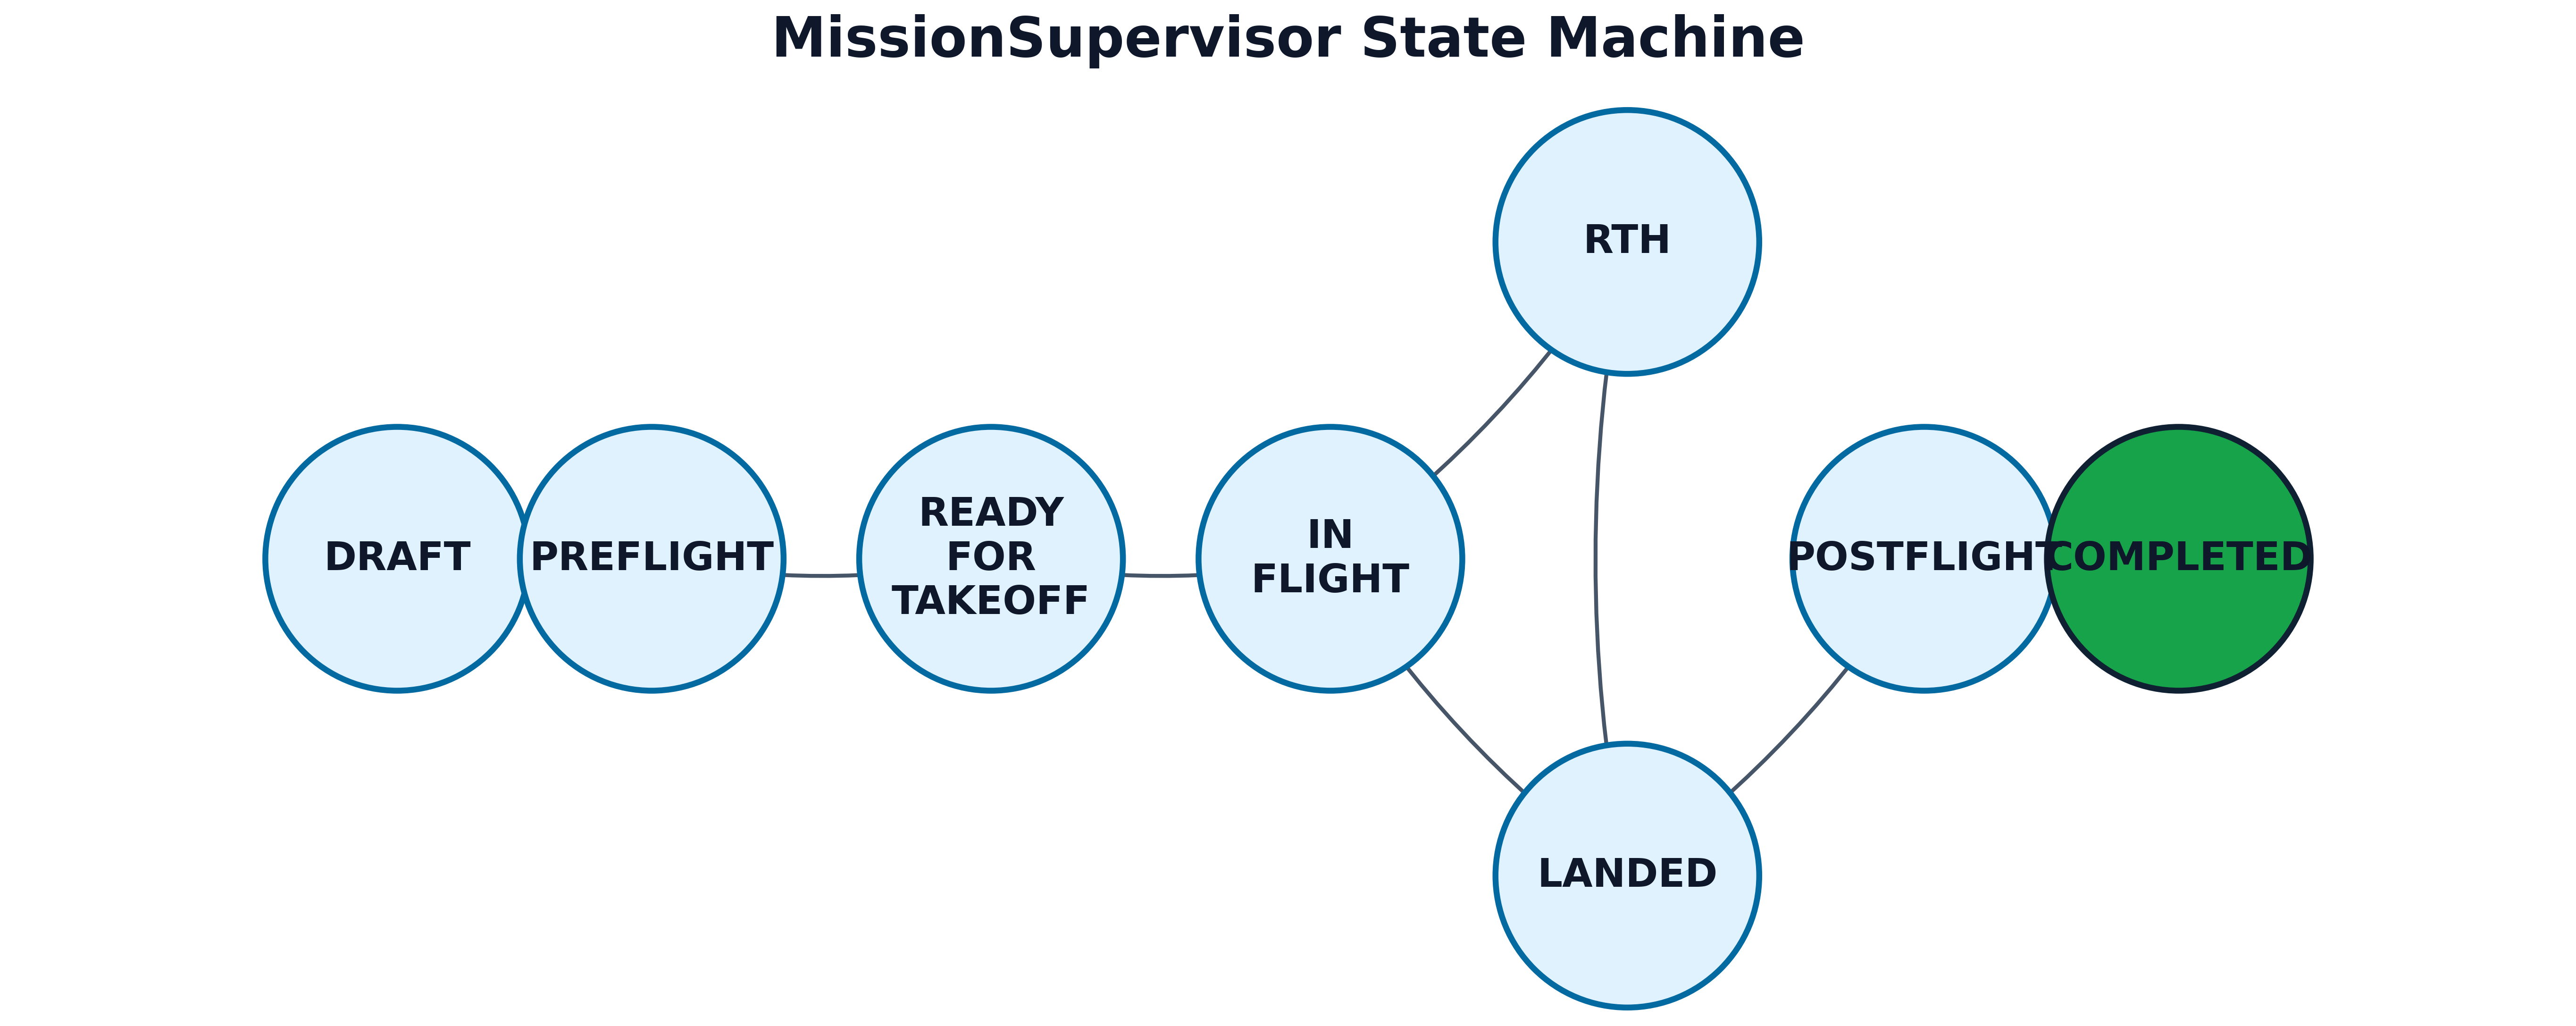
\includegraphics[width=0.45\textwidth]{supervisor_state_machine.png}
\caption{The MissionSupervisor State Machine, illustrating the progression from \textit{draft} through \textit{completed} states.}
\label{fig:statemachine}
\end{figure}

\subsection{FIPA-ACL Communication Protocol}
For the system to function deterministically, the agents must communicate using a standardized protocol. We adopted the Foundation for Intelligent Physical Agents (FIPA) Agent Communication Language (ACL) specifications \cite{b4}. 

As illustrated in Fig. \ref{fig:fipaflow}, the communication flow follows a strict request-response paradigm. The backend maintains an internal \texttt{fipa\_log} to record all transactions, ensuring that every multi-agent interaction is auditable and strictly typed by its performative:

\vspace{1em}
\noindent\textbf{Listing 1. FIPA-ACL Message Logging Implementation}
\begin{lstlisting}
def _fipa(self, sender: str, receiver: str, performative: str, content: str) -> None:
    self.fipa_log.append({
        "timestamp": utc_now(),
        "sender": sender,
        "receiver": receiver,
        "performative": performative,
        "content": content,
    })
\end{lstlisting}

For example, when telemetry indicates high wind, the Meteorology Agent issues a \textit{PROPOSE} message. The Mission Supervisor then evaluates this and may issue a \textit{REQUEST} to the Safety Officer for an emergency landing decision, culminating in an \textit{INFORM} message back to the operator interface.

\begin{figure}[H]
\centering
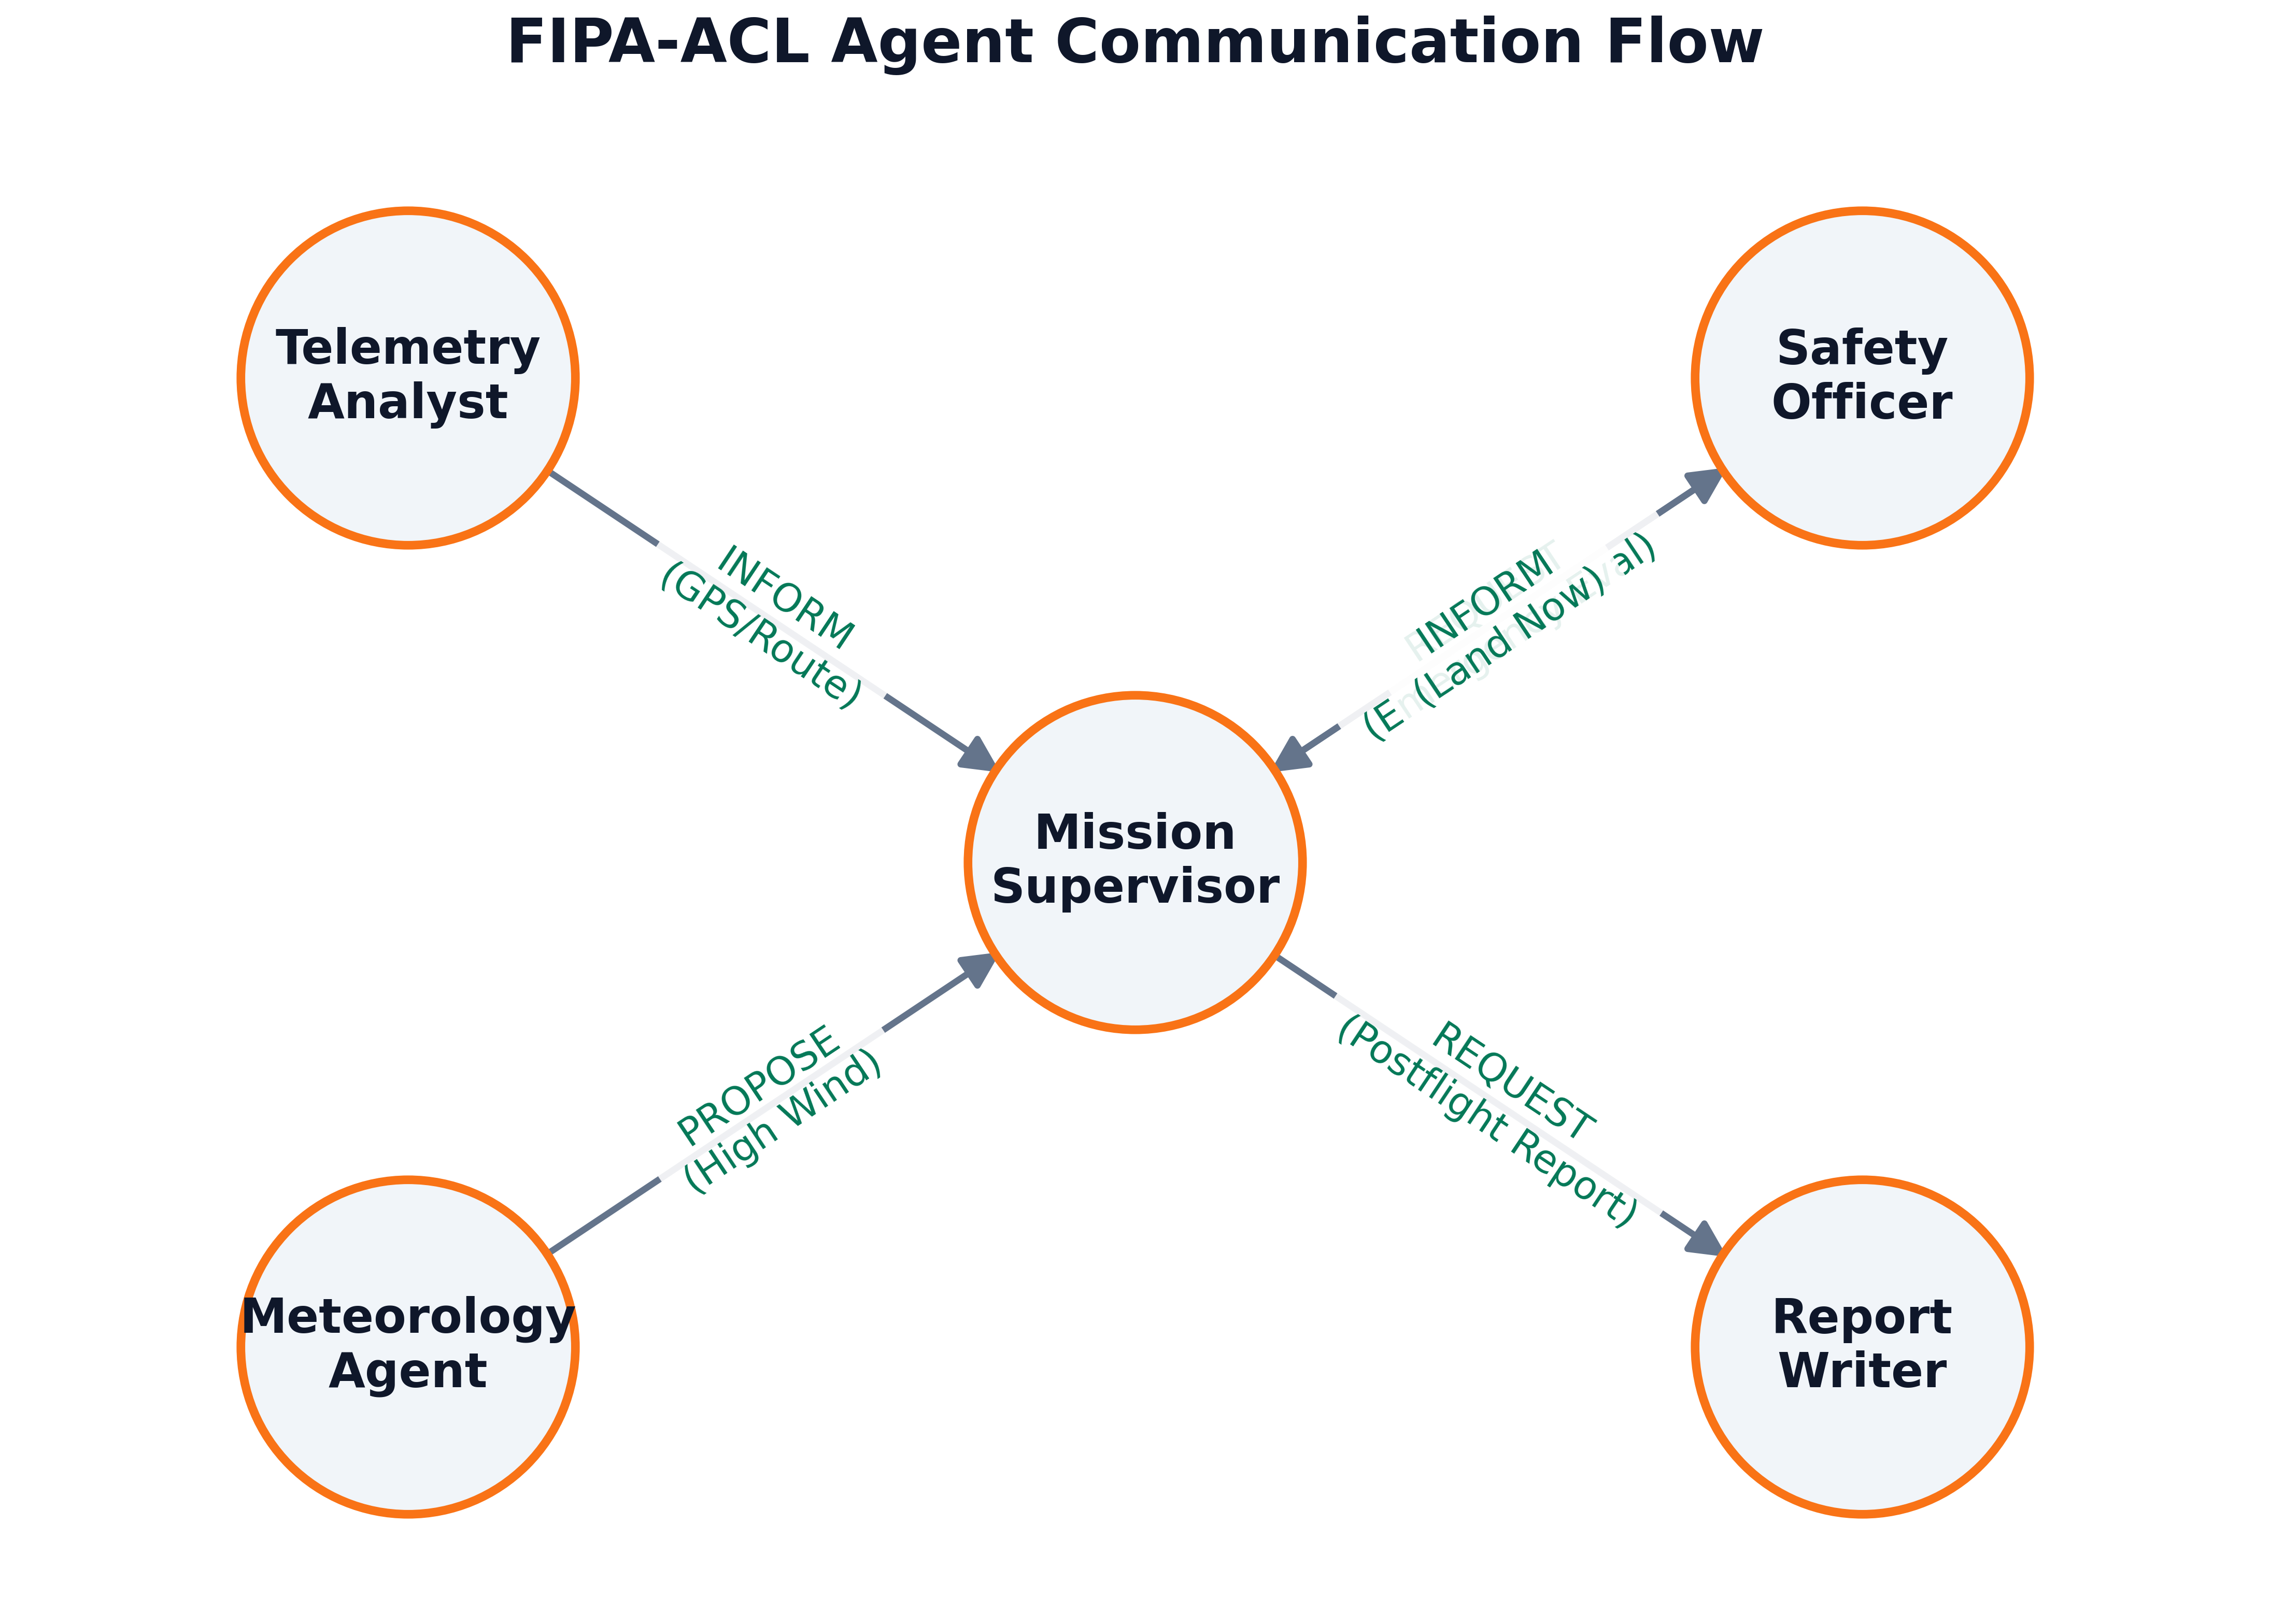
\includegraphics[width=0.45\textwidth]{fipa_communication_flow.png}
\caption{FIPA-ACL interactions among the UAV safety agents during a mission sequence.}
\label{fig:fipaflow}
\end{figure}

%% ============================================
%% 3. TELEMETRY AND AUTONOMOUS OVERSIGHT
%% ============================================
\section{Telemetry and Autonomous Oversight}

A critical vulnerability in traditional checklist applications is the assumption that the operator's input is invariably correct. An operator might manually check off "Weather Conditions are Optimal" despite rapidly changing wind speeds.

To address this, our system introduces a \texttt{TelemetryLogReader} that streams simulated flight logs containing real-time values (battery percentage, GPS satellite lock count, wind speed, and heading). The \texttt{process\_next\_event()} loop feeds these data points to the respective agents for proactive checks.

The agents are explicitly instructed with critical safety boundaries:
\begin{itemize}
    \item \textbf{Wind speed:} Must not exceed 12 m/s (NO-GO limit). Warnings are issued if wind reaches 9 m/s.
    \item \textbf{Battery level:} Must remain above 90\% for a safe mission buffer; if it falls lower during \textit{in\_flight}, the Safety Officer warns the operator to calculate RTH reserves.
    \item \textbf{GPS lock:} Warnings are issued by the Telemetry Analyst if satellite lock drops to 15 or below.
\end{itemize}

If any of these conditions are violated, the specialized agents autonomously override the manual checklist progression. The \textit{MissionSupervisor} evaluates these thresholds continuously as shown in Listing 2:

\vspace{1em}
\noindent\textbf{Listing 2. Autonomous Telemetry Risk Evaluation}
\begin{lstlisting}
def _risk_summary(self) -> dict:
    wind = self.telemetry_snapshot.get("wind")
    battery = self.telemetry_snapshot.get("battery")
    status = "GO"
    notes = []
    
    if wind is not None and wind >= 9:
        status = "WARNING"
        notes.append("Ruzgar sinira yaklasiyor.")
    if battery is not None and battery < 90:
        status = "WARNING" if status == "GO" else status
        notes.append("Batarya gorev sonuna yaklasiyor.")
        
    return {"status": status, "notes": notes}
\end{lstlisting}

They inject proactive alerts (e.g., "Wind early warning") into the operator's dashboard, creating a fail-safe mechanism where the system's logical deduction acts as a safety net against human error. This autonomous intervention logic is presented in Listing 3.

\vspace{1em}
\noindent\textbf{Listing 3. Proactive Autonomous Interventions}
\begin{lstlisting}
if wind is not None and wind >= 8:
    self._add_proactive(
        "wind-early-warning",
        "Meteorology Agent",
        "Ruzgar trendi yukseliyor",
        "Ruzgar limit yakini. Rota kisaltma veya erken inis icin hazirlik oneriliyor.",
        severity="warning",
        actions=["Rota kisalt", "RTH hazirla"],
    )
\end{lstlisting}

\begin{figure}[H]
\centering
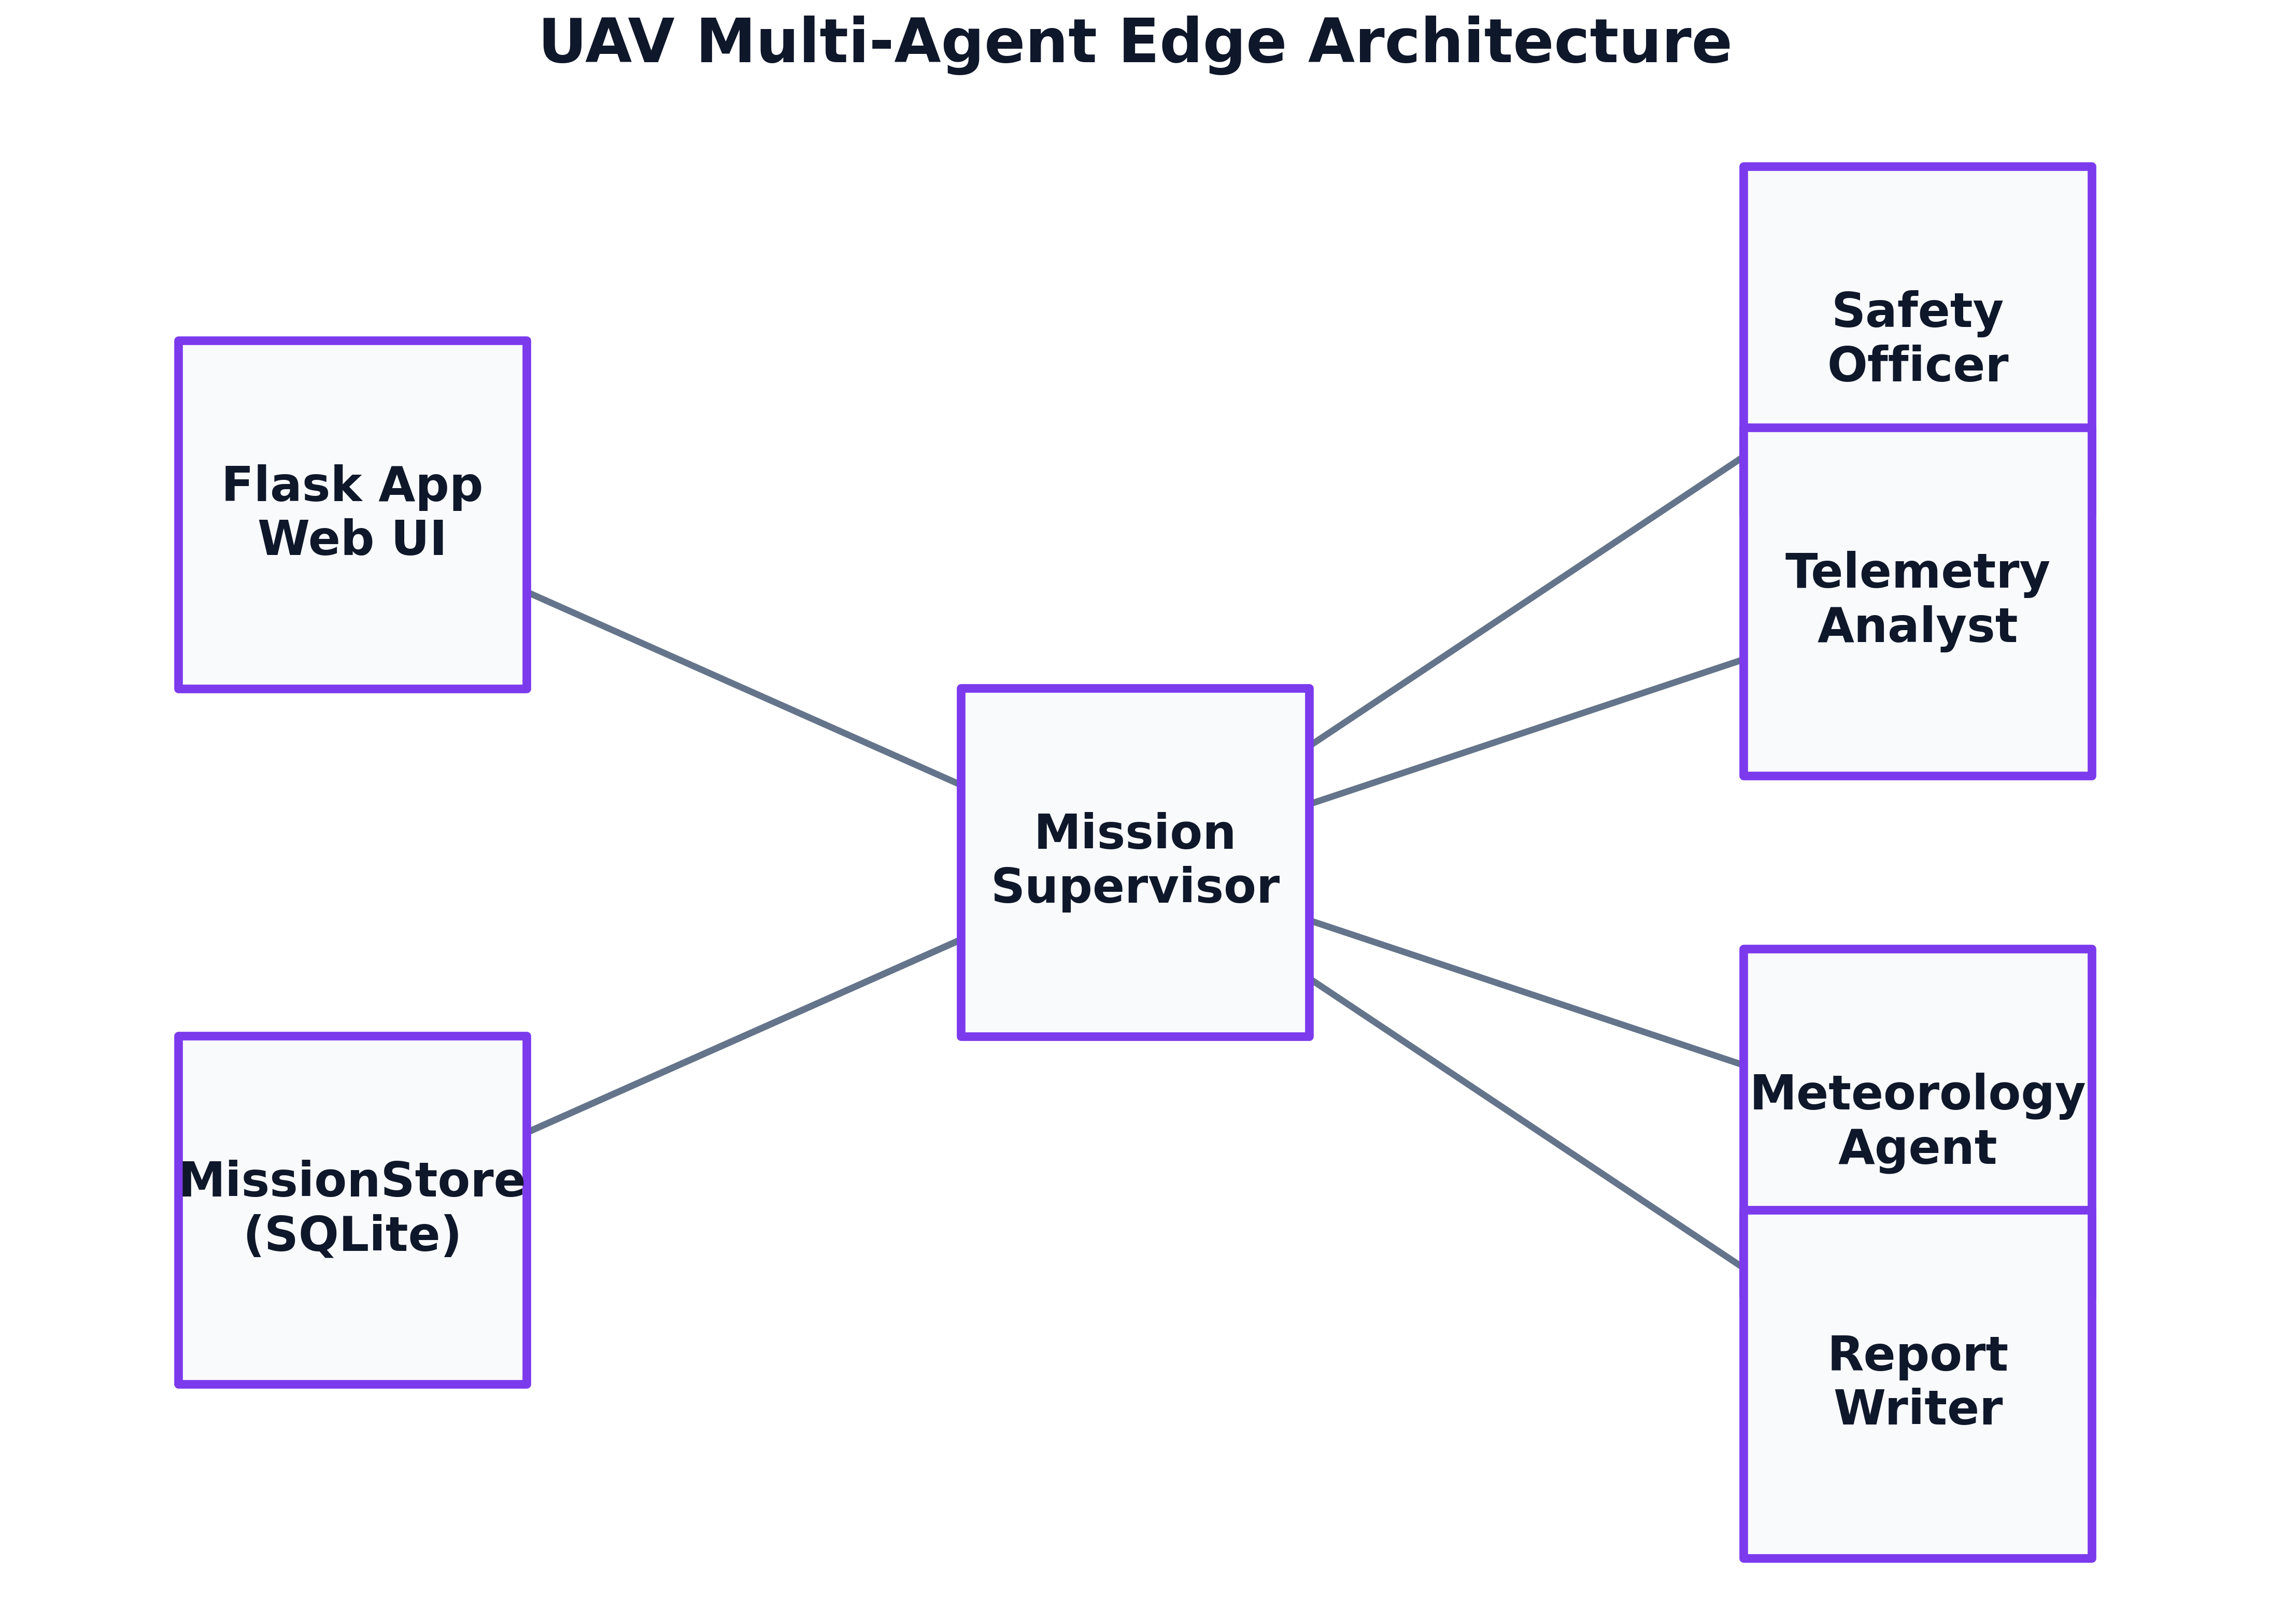
\includegraphics[width=0.45\textwidth]{mas_architecture.png}
\caption{The complete UAV Multi-Agent Edge Architecture, showing the interaction between the Flask UI, SQLite storage, and the internal Agent State Machine.}
\label{fig:architecture}
\end{figure}

%% ============================================
%% 4. CONCLUSION AND FUTURE WORK
%% ============================================
\section{Conclusion and Future Work}

This paper presented an autonomous Multi-Agent System designed to enhance UAV flight safety through the integration of state-machine-driven agent roles and real-time telemetry. By utilizing FIPA-ACL standards, we established a robust communication pipeline among specialized agents capable of cross-validating human inputs against live environmental data. 

Our implementation proves that multi-agent design patterns can transition from passive conversational bots to active, deterministic decision-makers in safety-critical domains. Future work will focus on integrating edge-based, locally hosted LLMs to provide real-time cognitive reasoning over the simulated FIPA-ACL logs, eliminating the latency and connectivity constraints associated with cloud-based API inference.

\begin{thebibliography}{00}
\bibitem{b1} R. Austin, \textit{Unmanned Aircraft Systems: UAVS Design, Development and Deployment}. Wiley, 2010.
\bibitem{b2} T. Brown et al., "Language Models are Few-Shot Learners," \textit{Advances in Neural Information Processing Systems}, vol. 33, pp. 1877-1901, 2020.
\bibitem{b3} M. Wooldridge, \textit{An Introduction to MultiAgent Systems}. John Wiley \& Sons, 2009.
\bibitem{b4} FIPA, "FIPA ACL Message Structure Specification," \textit{Foundation for Intelligent Physical Agents}, SC00061G, 2002.
\end{thebibliography}

\end{document}
